\DiaryEntry{Kalman Filter, 1}{2019-06-06}{Stochastic}

\subsection{Introduction}

The entry \ref{2017-02-01:entry} considered the posterior distribution of Gaussian RVs. In particular, a random vector $\xbf$ has distribution

\bee
p(\xbf) = \Nc(\xbf|\hat\xbf, \Sigmabf)
\eee

The random vector $\ybf$ is observed according to

\bee
\ybf = \Gbf \xbf + \vbf, \quad \vbf \sim \Nc(\zerobf, \Rbf)
\eee

and therefore has the following conditional distribution

\bee
p(\ybf | \xbf) = \Nc(\ybf | \Gbf \xbf, \Rbf)
\eee

The posterior distribution of $\xbf | \ybf$ is then given according to

\bee
p(\xbf | \ybf) = \Nc(\xbf | \hat\xbf + \Sigmabf \Gbf^T (\Gbf \Sigmabf \Gbf^T + \Rbf )^{-1} (\ybf - \Gbf \hat\xbf), \Sigmabf - \Sigmabf \Gbf^T (\Gbf \Sigmabf \Gbf^T + \Rbf)^{-1} \Gbf \Sigmabf
\eee

The posterior mean is a mixture of the prior $\hat\xbf$ and the scaled difference $(\ybf - \Gbf \hat\xbf)$. In the extreme case of perfect prior knowledge $\Sigmabf \rightarrow \zerobf$, we have

\bee
\lim_{\Sigmabf \rightarrow \zerobf} \hat\xbf + \Sigmabf \Gbf^T (\Gbf \Sigmabf \Gbf^T + \Rbf )^{-1} (\ybf - \Gbf \hat\xbf) = \hat\xbf
\eee

i.e. the prior information alone is considered. In the other extreme case of perfect observation $\Rbf \rightarrow \zerobf$, we have

\bee
\lim_{\Rbf \rightarrow \zerobf} \hat\xbf + \Sigmabf \Gbf^T (\Gbf \Sigmabf \Gbf^T + \Rbf )^{-1} (\ybf - \Gbf \hat\xbf) = \hat\xbf + \Sigmabf \Gbf^T (\Gbf \Sigmabf \Gbf^T)^{-1} (\ybf - \Gbf \hat\xbf) = \hat\xbf + \Gbf^{-1} (\ybf - \Gbf \hat\xbf) = \Gbf^{-1} \ybf
\eee

i.e. the observation alone is considered.

\paragraph{Impact of Correlation.} Assume that $\xbf$ is zero-mean and uncorrelated,

\bee
\xbf \sim \Nc(\zerobf, \Ibf)
\eee

we observe both components ($\Gbf = \Ibf$) with uncorrelated noise ($\Rbf = 0.1 \Ibf$). Then the posterior covariance matrix is

\bee
\Sigmabf - \Sigmabf \Gbf^T (\Gbf \Sigmabf \Gbf^T + \Rbf)^{-1} \Gbf \Sigmabf \approx \begin{pmatrix} 0.0909091  & 0.0 \\ 0.0 & 0.0909091\end{pmatrix}
\eee

The error is uncorrelated and has variance slighlty less than the noise variance; this is because the prior information reduces the estimator variance. Now let's see what happens if $\xbf$ is highly correlated,

\bee
\xbf \sim \Nc(\zerobf, \begin{pmatrix} 1.0 & 0.9999 \\ 0.9999 & 1.0 \end{pmatrix})
\eee

The observation $\Gbf$ and $\Rbf$ are the same as above and we have

\bee
\Sigmabf - \Sigmabf \Gbf^T (\Gbf \Sigmabf \Gbf^T + \Rbf)^{-1} \Gbf \Sigmabf \approx \begin{pmatrix} 0.0476689 & 0.047569 \\ 0.047569 & 0.0476689  \end{pmatrix}
\eee

In this case the variance is approx. half the noise variance. This makes sense, as both $\xbf$ components are the same (because of the high correlation) and we effectively observe the same value twice, thereby reducing the variance by half.


\subsection{Kalman Filter}

The Kalman filter solves the problem of estimating a sequence of hidden RVs, $\{ \xbf_k \}$ from a sequence of (noisy) observations, $\{ \ybf_k \}$. The sequence of $\{ \xbf_k \}$ is described by a state space equation,

\bee
\xbf_{k+1} = \Abf \xbf_k + \wbf_{k+1}, \quad \wbf_k \sim \Nc(\zerobf, \Qbf)
\eee

and the "model noise" $\wbf_k$ being independent for different $k$, $E\{\wbf_k \wbf_l\} = \Qbf \delta_{k,l}$. At time $k=1$, the system is in an initial state, given by the prior $\xbf_1 \sim \Nc(\hat \xbf_1, \Sigmabf_1)$. The observations are given by

\bee
\ybf_k = \Gbf \xbf_k + \vbf, \quad \vbf_k \sim \Nc(\zerobf, \Rbf)
\eee

with the observation noise $\vbf$ being independent for different $k$, $E\{\wbf_k \wbf_l\} = \Qbf \delta_{k,l}$.

\paragraph{Principle of Operation.} Upon observation of $\ybf_1$, the Kalman filter treats its knowledge of $\hat \xbf_1$ and $\Sigmabf_1$ as prior and calculates the posterior density which is a Gaussian with mean $\hat\xbf_1^F$ and covariance matrix $\Sigmabf_1^F$. This is called the \emph{filtering step} of the filter. The posterior density is then used in the \emph{prediction step} to form an estimate for $\xbf_2$ in the form of the mean $\hat\xbf_2^P$ and covariance matrix $\Sigmabf_2^P$.

After observing $\ybf_2$, the filter uses the predictions $\hat\xbf_2^P$ and $\Sigmabf_2^P$ as prior and performs a filtering and prediction step. The filter continues this process.

\paragraph{Filtering Step.} Our prior for $\xbf$ is $\Nc(\hat\xbf_1, \Sigmabf_1)$ and from the previous Subsection we know

\bee
\xbf_1 | \ybf_1 \sim \Nc(\xbf_1^F, \Sigmabf_1^F)
\eee

with posterior mean

\bee
\xbf_1^F = \hat\xbf_1 + \Sigmabf_1 \Gbf^T (\Gbf \Sigmabf_1 \Gbf^T + \Rbf)^{-1} (\ybf_1 - \Gbf \hat\xbf_1)
\eee

and covariance matrix

\bee
\Sigmabf_1^F = \Sigmabf_1 - \Sigmabf_1 \Gbf^T (\Gbf \Sigmabf_1 \Gbf^T + \Rbf)^{-1} \Gbf \Sigmabf_1
\eee

\paragraph{Prediction Step.} Now we use the state space equations to obtain a prediction for $\xbf_2$. Since everything is Gaussian, we have

\bee
\xbf_2 | \ybf_1 \sim \Nc(\hat\xbf_2^P, \Sigmabf_2^P) = \Nc(\Abf \xbf_1^F, \Abf \Sigmabf_1^F \Abf^T + \Qbf)
\eee


\subsection{Results}

We consider movement of a particle with unknown (i.e. to be estimated) velocity. The state vector $\xbf$ contains the position and the velocity of the particle

\bee
\xbf = \begin{pmatrix} x \\ \dot x \end{pmatrix} 
\eee

and the state update equation are given by

\bee
\begin{pmatrix} x_{k+1} \\ \dot x_{k+1} \end{pmatrix} = \begin{pmatrix} x_{k} + \dot x_k \\ \dot x_{k} \end{pmatrix} + \wbf_{k+1}
\eee

with state space update matrix

\bee
\Abf = \begin{pmatrix} 1 & 1 \\ 0 & 1 \end{pmatrix}
\eee

We do not observe the velocity, only the position $x$, therefore $\Gbf$ has the following form

\bee
\Gbf = \begin{pmatrix} 1 & 0 \end{pmatrix}
\eee

The covariance matrices are given by

\bee
\Qbf = \begin{pmatrix} 0.1 & 0 \\ 0 & 0.001 \end{pmatrix}, \quad \Rbf = \begin{pmatrix} 0.01 \end{pmatrix}
\eee

i.e. there is "some" random change in position, but a smaller random change in the (unknown) velocity.

For the simulation we started with a velocity of $\dot x = 1$ for $k<25$ and then increased the velocity to $\dot x=5$. We first show a plot of the true (red) vs the estimated (filtered) position (blue). The stimate follows the true value quite closely.

\begin{figure}[hbt!]
\centering
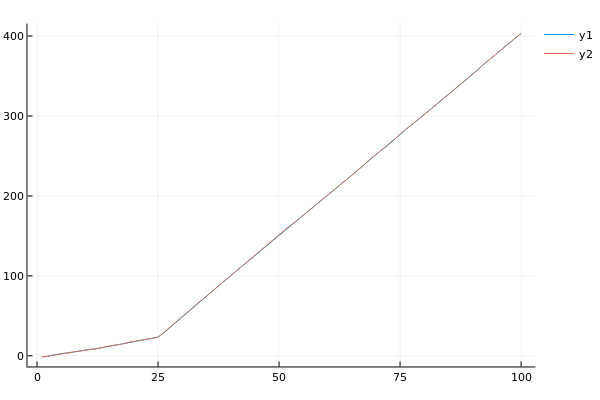
\includegraphics[scale=0.5]{images/kalman_1_1.png}
\end{figure}

Next, we show a plot of the true (red) vs estimated (filtered) velocity (blue). After the velocity step it takes about 25 time steps for the estimate to reach the new velocity.


\begin{figure}[hbt!]
\centering
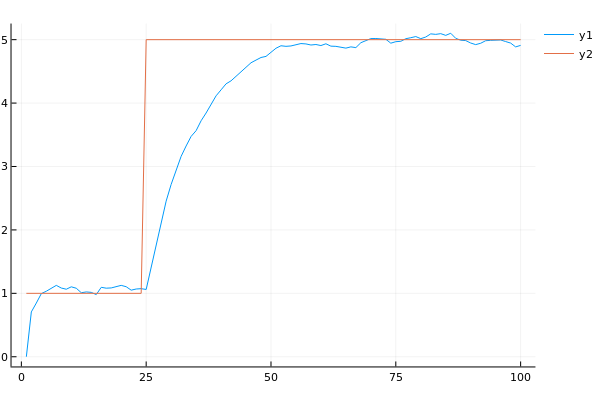
\includegraphics[scale=0.5]{images/kalman_1_2.png}
\end{figure}


%%% Local Variables:
%%% mode: latex
%%% TeX-master: "journal"
%%% End:
